\section{Interface user guide}
\label{interface}
\noindent
\subsection{How to design a mission}
After the user run the user interface software, a window as the one seen in fig. \ref{IDE_overall_design} will appear, on left side of the screen is the mission chose and line chose bar, user can drag tasks from here and drop them onto the white section on the right and use the straight line and curve line connect all the missions together, after enter the IP address and the port number and pressed  the TCP communication button, the server will receive a JSON string as seen in \ref{IDE_overall_design3}.
\begin{figure}[!ht]
	\begin{center}
		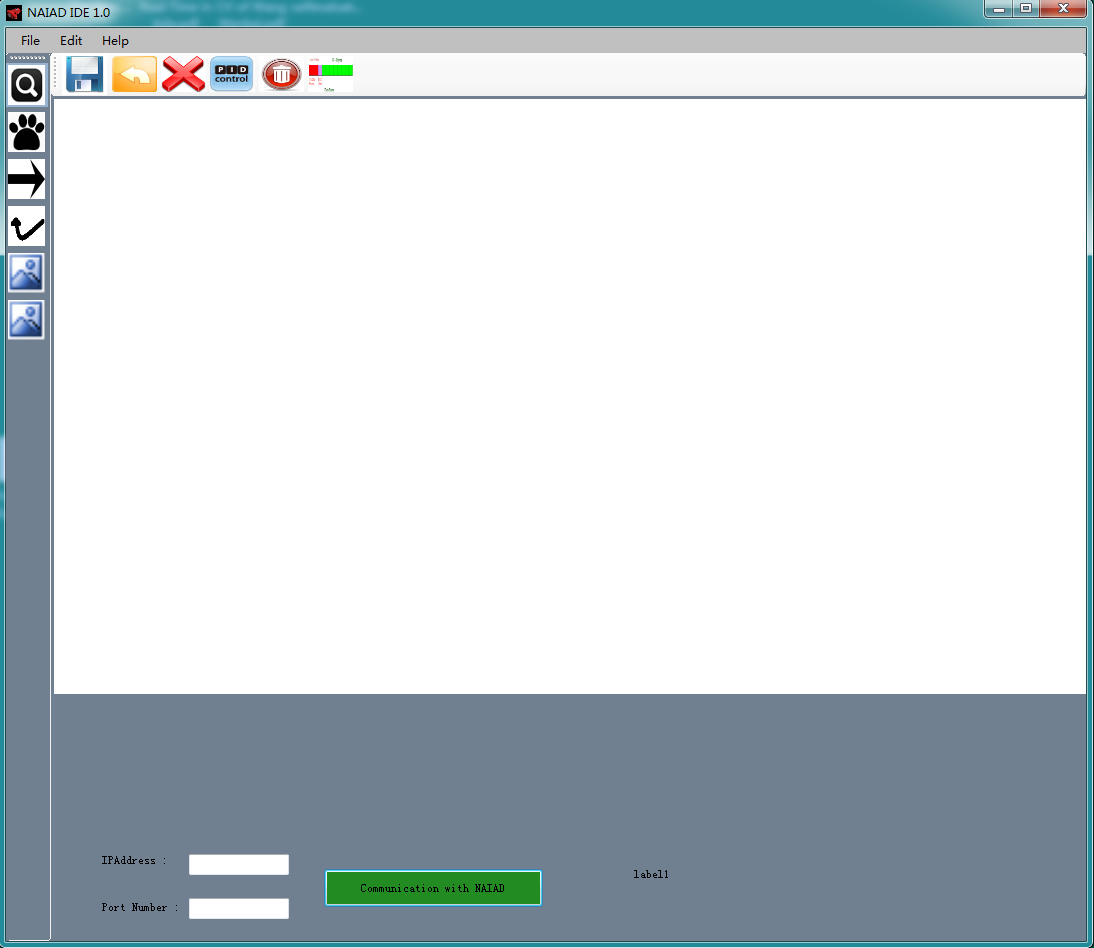
\includegraphics[width=80mm]{./Images/Software/over_all_view_of_the_panel.png}
		\caption{The over all view of the panel}
		\label{IDE_overall_design}
	\end{center}
\end{figure}
\begin{figure}[!ht]
	\begin{center}
		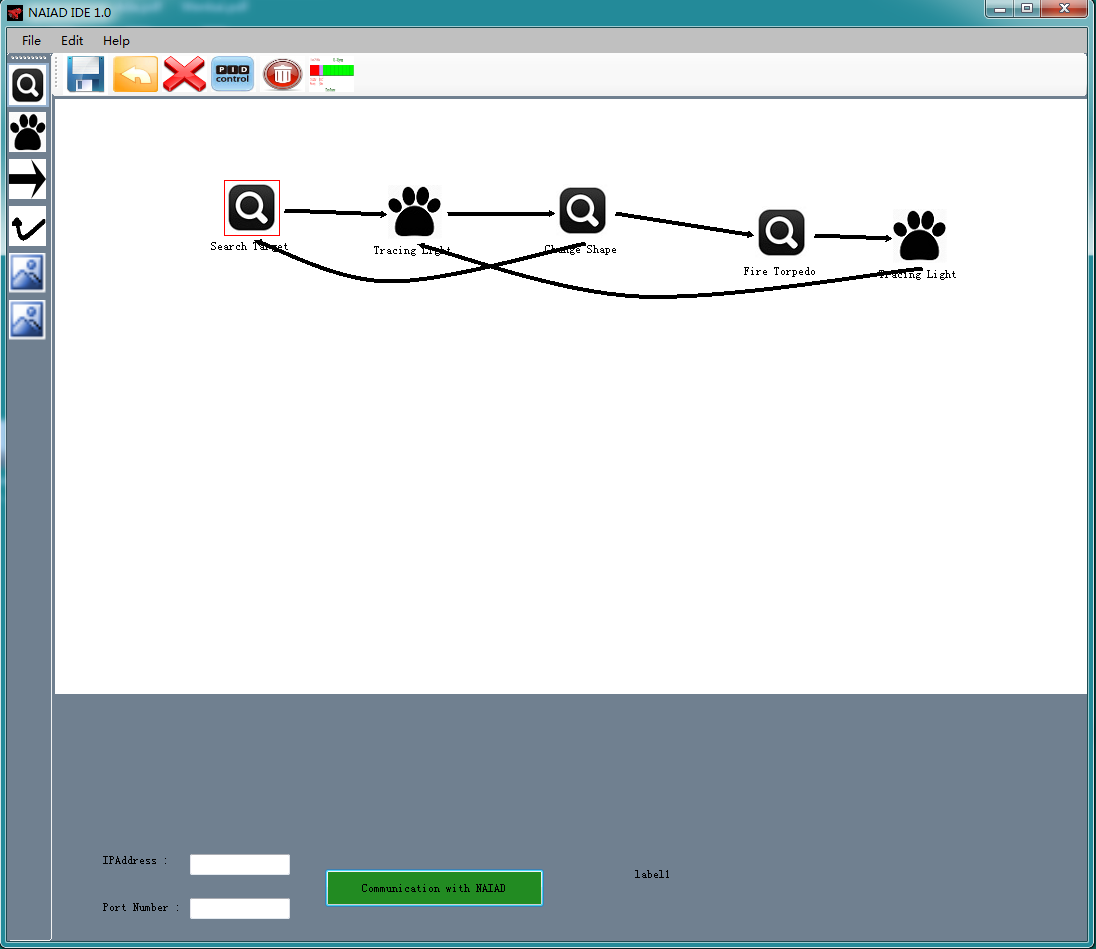
\includegraphics[width=80mm]{./Images/Software/Example_of_how_to_use.png}
		\caption{A example about how to use the interface}
		\label{IDE_overall_design2}
	\end{center}
\end{figure}
\begin{figure}[!ht]
	\begin{center}
		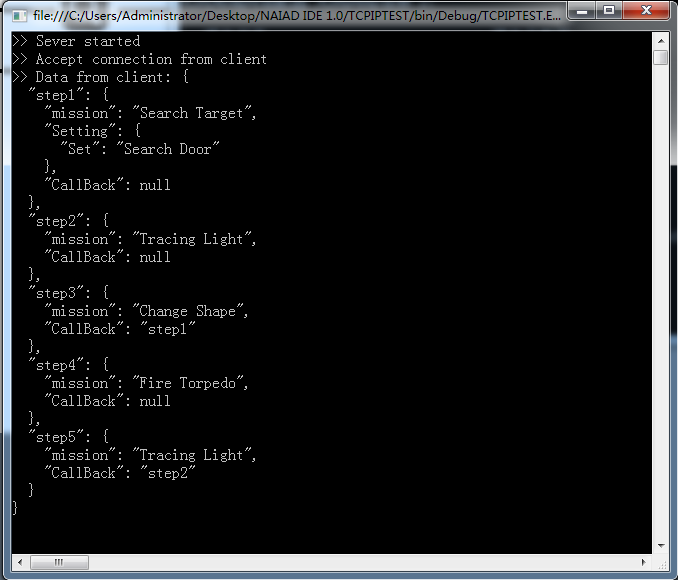
\includegraphics[width=80mm]{./Images/Software/Json_string_result.png}
		\caption{The output of the json string}
		\label{IDE_overall_design3}
	\end{center}
\end{figure}

\subsection{PID control}
When the user pressed the PID control part, an window as seen in fig. \ref{IDE_overall_design4} will appear, the user can set the PID value on position X, position Y and position Z. After that user can set the PID value for the orientation yaw, pitch and roll. When finished all the setting, there are three buttons that the user can chose: save button, import button and TCP communication button.
\begin{figure}[!ht]
	\begin{center}
		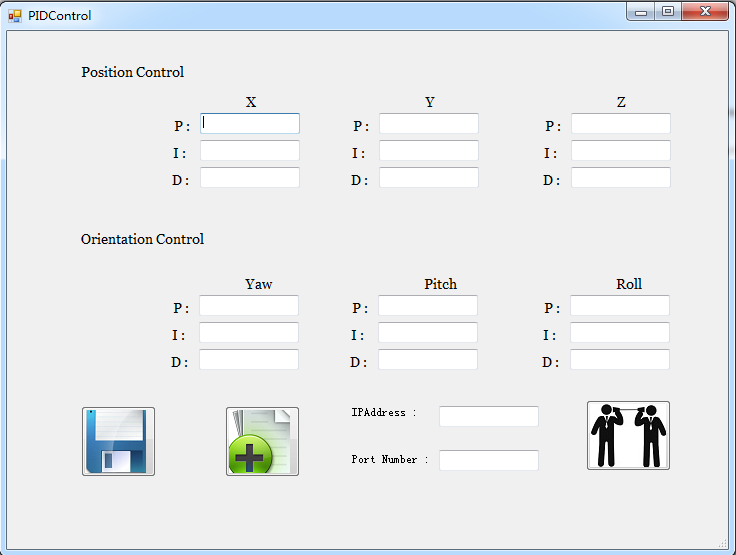
\includegraphics[width=80mm]{./Images/Software/PIDcontrol_part.png}
		\caption{The PID control setting part}
		\label{IDE_overall_design4}
	\end{center}
\end{figure}

\subsection{CAN message setting}
After pressed the CAN message button, the user will see a window as seen in fig. \ref{IDE_overall_design5}, there user can set the ID of the CAN message and the value for different byte. After that user need enter the IP address and the port number, then all the information will be sent to Naiad.
\begin{figure}[!ht]
	\begin{center}
		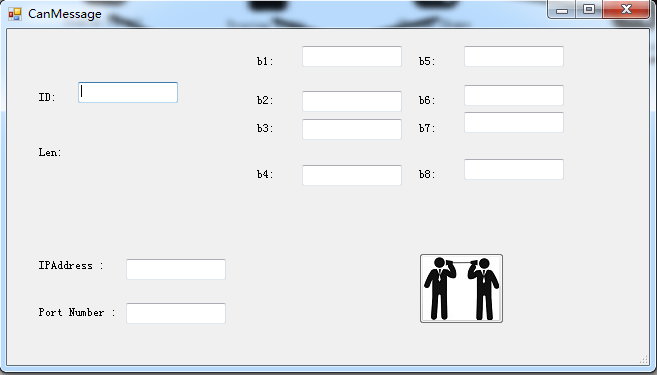
\includegraphics[width=80mm]{./Images/Software/CANmessage_part.png}
		\caption{The CAN message setting part}
		\label{IDE_overall_design5}
	\end{center}
\end{figure}
\subsection{About Naiad}
When the user click the Help button,there are two options to chose, Welcome button and About button, after you click any one of them, a window as seen in fig. \ref{IDE_overall_design6} will appear, there you can find the basic things about Naiad and the website.
\begin{figure}[!ht]
	\begin{center}
		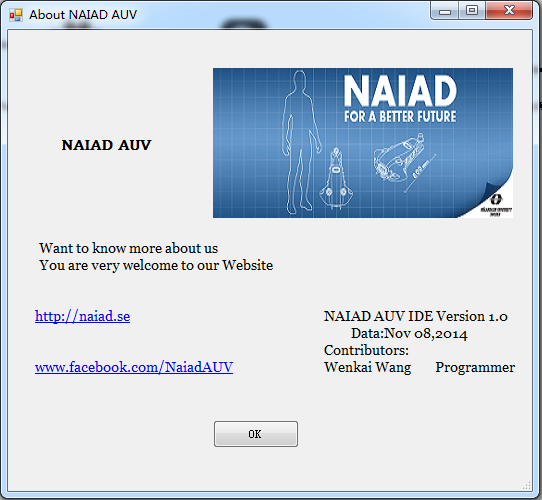
\includegraphics[width=80mm]{./Images/Software/about_part.png}
		\caption{The About part}
		\label{IDE_overall_design6}
	\end{center}
\end{figure}